%% Overleaf version: compiles on its own (pdfLaTeX, no BibTeX). GENERATED by manuscript/make_overleaf.py
\documentclass[journal=jctcce,manuscript=suppinfo]{achemso}
\usepackage[T1]{fontenc}
\usepackage{amsmath}
\usepackage{booktabs}
\usepackage{graphicx}
\usepackage{float}
\usepackage{placeins}
\usepackage[colorlinks=true,linkcolor=blue,citecolor=blue,urlcolor=blue]{hyperref}
\setkeys{acs}{articletitle=true,doi=true}
\newcommand*{\rows}[1]{\csname @@input\endcsname #1 }  % expandable \input for table bodies (before \bottomrule)
\renewcommand{\thesection}{S\arabic{section}}
\renewcommand{\thetable}{S\arabic{table}}
\renewcommand{\thefigure}{S\arabic{figure}}
\renewcommand{\theequation}{S\arabic{equation}}

% Every table body is \rows{...} from ../codes/results, written by the standalone scripts in ../codes (copied by build.sh).

\title{Probing Dimensional Crossover in SCAN Exchange with Exact Quasi-One-Dimensional Wires and Quasi-Two-Dimensional Sheets}
\author{Gabriel Chirchir}
\author{Subrata Jana}
\author{Szymon \'Smiga}
\affiliation{Institute of Physics, Faculty of Physics, Astronomy and Informatics,
Nicolaus Copernicus University in Toru\'n, ul.~Grudzi\c{a}dzka~5, 87-100 Toru\'n, Poland}

\usepackage{xcolor}
% new-result highlighting (user 2026-11-05): \novelty{...} prints red; for the final
% submission change {red} to {black} here (one line) to remove all highlighting
\newcommand{\novelty}[1]{{\color{red}#1}}
% Figures: names are unique to this paper (scan1d2d_*.pdf). Overleaf compiles from the project root, so if
% this folder sits inside a larger Overleaf project under a name not listed here, add {<folder>/figures/}.
\graphicspath{{figures/}{overleaf/figures/}{scan/figures/}{SCAN_1D_2D/figures/}{scan_1d_2d/figures/}{dcscan/figures/}{DC-SCAN/figures/}{scan1d2d/figures/}}
\begin{document}

All results are fixed-density and exchange-only; no self-consistent
calculation is involved.  Every equation of the DC-SCAN construction is in
Appendix~\href{main.pdf\#section*.6}{A} of the main text and is cited here by its main-text
number.  Section~\ref{sec:anigto-derivation} derives the aniGTO integrals and
density derivatives used for the exact references, and
Section~\ref{sec:codes} lists the standalone scripts that produce every table
and figure.

\section{aniGTO integrals and density derivatives used in this work}
\label{sec:anigto-derivation}
This section derives the quantities taken from the aniGTO anisotropic
Gaussian package\cite{chirchir2026anigto}; the corresponding functions are
copied verbatim into the scripts of Section~\ref{sec:codes}.

\subsection{Anisotropic Cartesian Gaussians and the harmonic-trap basis}
An aniGTO primitive has one exponent per Cartesian axis,
\begin{equation}
g_{\mathbf l}(\mathbf r;\mathbf a,\mathbf A)=\prod_{k=x,y,z}(x_k-A_k)^{l_k}\,e^{-a_k(x_k-A_k)^2},
\label{eq:ani-prim}
\end{equation}
and the normalized $s$ function ($\mathbf l=0$) is $N_s\,g_0$ with
\begin{equation}
N_s=\prod_k\Bigl(\frac{2a_k}{\pi}\Bigr)^{1/4}.
\label{eq:ani-norm}
\end{equation}
The harmonic-trap (``dot'') basis for the trap frequencies
$\boldsymbol\omega=(\omega_x,\omega_y,\omega_z)$ uses $a_k=\omega_k/2$, so its
$s$ function is the ground state of the anisotropic oscillator.  Doubly
occupied, it gives
\begin{equation}
n(\mathbf r)=2N_s^2\,e^{-\sum_k\omega_kx_k^2}=n_A(\mathbf r),\qquad A=\mathrm{diag}(\boldsymbol\omega),
\label{eq:ani-density}
\end{equation}
which is the reference density of eqs~\href{main.pdf\#equation.7}{A7} and
\href{main.pdf\#equation.8}{A8} for $\boldsymbol\omega=(1,1,\lambda^2)$ (sheet) and
$(\lambda^2,\lambda^2,1)$ (wire).  The excited trap functions along $z$ are the
Hermite functions,
\begin{equation}
h_0(z)=\pi^{-1/4}e^{-z^2/2},\quad h_1=\sqrt2\,z\,h_0,\quad
h_k=\sqrt{\frac{2}{k}}\,z\,h_{k-1}-\sqrt{\frac{k-1}{k}}\,h_{k-2},
\label{eq:ani-hermite}
\end{equation}
so the $N=4$ and $N=6$ wires of Section~\ref{sec:dcscan-beyond} occupy
$\phi_k=g(\rho)h_k(z)$, $k<N/2$, with
$g^2(\rho)=(\lambda^2/\pi)e^{-\lambda^2\rho^2}$: the $s$, $p_z$ and $d_{zz}$
trap functions.

\subsection{One-dimensional building blocks}
Along each axis the product of two Gaussians is one Gaussian (Gaussian
product theorem),
\begin{equation}
e^{-a(x-A)^2}e^{-b(x-B)^2}=E_{AB}\,e^{-p(x-P)^2},\qquad
p=a+b,\quad P=\frac{aA+bB}{p},\quad E_{AB}=e^{-\frac{ab}{p}(A-B)^2},
\label{eq:ani-gpt}
\end{equation}
and every remaining integral reduces to the Gaussian moments
\begin{equation}
\int_{-\infty}^{\infty}x^m e^{-\beta x^2}dx=
\begin{cases}\sqrt{\pi/\beta}\;(m-1)!!\,(2\beta)^{-m/2}, & m\ \text{even},\\
0, & m\ \text{odd},\end{cases}
\label{eq:ani-moment}
\end{equation}
with $(-1)!!=1$.  Products of shifted monomials are expanded binomially
about the product centre $U$,
\begin{equation}
\int\prod_{i=1}^{4}(x-X_i)^{n_i}e^{-\beta(x-U)^2}dx
=\sum_{j_1\ldots j_4}\prod_{i}\binom{n_i}{j_i}(U-X_i)^{n_i-j_i}
\int x^{j_1+j_2+j_3+j_4}e^{-\beta x^2}dx .
\label{eq:ani-int2}
\end{equation}

\subsection{Two-electron repulsion integral}
With the Gaussian transform of the Coulomb operator (eq~\href{main.pdf\#equation.43}{A43}
with integration variable $u$),
\begin{equation}
\frac{1}{r_{12}}=\frac{2}{\sqrt\pi}\int_0^\infty e^{-u^2r_{12}^2}du,
\label{eq:ani-coulomb}
\end{equation}
the six-dimensional integral over $\mathbf r_1,\mathbf r_2$ separates into
three one-dimensional factors for every $u$:
\begin{equation}
(ab|cd)=\frac{2}{\sqrt\pi}\,E_{AB}E_{CD}\int_0^\infty du\prod_{k=x,y,z}I_k(u^2),
\label{eq:ani-eri-u}
\end{equation}
\begin{equation}
I_k(u^2)=\iint(x_1-A)^{n}(x_1-B)^{m}(x_2-C)^{p}(x_2-D)^{q}\,
e^{-p_{ab}(x_1-P)^2}e^{-p_{cd}(x_2-Q)^2}e^{-u^2(x_1-x_2)^2}dx_1dx_2,
\label{eq:ani-Ik}
\end{equation}
where $p_{ab},P$ and $p_{cd},Q$ come from eq~\ref{eq:ani-gpt} for the pairs
$(a,b)$ and $(c,d)$ along axis $k$.  The $x_1$ integral is done first:
completing the square,
\begin{equation}
e^{-p_{ab}(x_1-P)^2-u^2(x_1-x_2)^2}=e^{-(p_{ab}+u^2)(x_1-X)^2}\,e^{-\xi(x_2-P)^2},\qquad
X=\frac{p_{ab}P+u^2x_2}{p_{ab}+u^2},\quad \xi=\frac{p_{ab}u^2}{p_{ab}+u^2},
\label{eq:ani-x1}
\end{equation}
and shifting $x_1=y+X$ turns $x_1-A$ into
$y+\frac{u^2}{p_{ab}+u^2}(x_2-A')$ with
$A'=[A(p_{ab}+u^2)-p_{ab}P]/u^2$ (likewise $B'$).  Expanding binomially and
using eq~\ref{eq:ani-moment} for $y$ gives
\begin{multline}
I_k(u^2)=\sqrt{\frac{\pi}{p_{ab}+u^2}}\sum_{i\le n,\,j\le m}^{i+j\ \mathrm{even}}
\binom{n}{i}\binom{m}{j}\frac{(i+j-1)!!}{[2(p_{ab}+u^2)]^{(i+j)/2}}
\Bigl(\frac{u^2}{p_{ab}+u^2}\Bigr)^{n+m-i-j}
e^{-\frac{p_{cd}\xi}{p_{cd}+\xi}(P-Q)^2}\\
\times\int(x_2-A')^{n-i}(x_2-B')^{m-j}(x_2-C)^{p}(x_2-D)^{q}
e^{-(p_{cd}+\xi)(x_2-U)^2}dx_2,
\qquad U=\frac{p_{cd}Q+\xi P}{p_{cd}+\xi},
\label{eq:ani-Ik-closed}
\end{multline}
and the last integral is eq~\ref{eq:ani-int2} with $\beta=p_{cd}+\xi$.
Eq~\ref{eq:ani-Ik-closed} is the aniGTO kernel \texttt{integral3}; it is
closed-form in $u^2$, so only the $u$ integral of eq~\ref{eq:ani-eri-u} is
numerical.

\paragraph{Default quadrature.}  aniGTO maps $u\in[0,\infty)$ to
$t=u/\sqrt{1+u^2}\in[0,1)$, with $u^2=t^2/(1-t^2)$ and
$du=(1-t^2)^{-3/2}dt$:
\begin{equation}
(ab|cd)=\frac{2}{\sqrt\pi}\,E_{AB}E_{CD}\int_0^1\frac{dt}{(1-t^2)^{3/2}}
\prod_kI_k\!\Bigl(\frac{t^2}{1-t^2}\Bigr),
\label{eq:ani-eri-t}
\end{equation}
evaluated by adaptive quadrature (\texttt{scipy.integrate.quad}, relative and
absolute tolerances $10^{-16}$).  For an exponent ratio $\rho_a$ the integrand
peaks at $u^2\sim\rho_a$, i.e.\ $1-t\approx1/(2\rho_a)$, which is the origin of
the default-quadrature errors of Tables~\ref{tab:dcscan-check} and
\href{main.pdf\#table.4}{4}.  The logarithmic variable $s=\ln u$ of
eq~\href{main.pdf\#equation.1}{1} integrates the same integrand of
eq~\ref{eq:ani-eri-u} with $du=e^{s}ds$.

\paragraph{Self-repulsion of one $s$ Gaussian.}  For four identical $s$
functions at the origin with exponents $a_k$, $p_{ab}=p_{cd}=2a_k$, $P=Q=0$
and $E_{AB}=E_{CD}=1$, so eq~\ref{eq:ani-Ik-closed} has only the $i=j=0$ term:
\begin{equation}
I_k(u^2)=\sqrt{\frac{\pi}{2a_k+u^2}}\sqrt{\frac{\pi}{2a_k+\xi}}
=\frac{\pi}{2\sqrt{a_k(a_k+u^2)}},\qquad \xi=\frac{2a_ku^2}{2a_k+u^2},
\label{eq:ani-Ik-s}
\end{equation}
because $(2a_k+u^2)(2a_k+\xi)=4a_k(a_k+u^2)$.  With $N_s^4=\prod_k2a_k/\pi$
and $A_k=2a_k$ (eq~\ref{eq:ani-density}),
\begin{equation}
(\phi\phi|\phi\phi)=N_s^4\,\frac{2}{\sqrt\pi}\int_0^\infty du\prod_k\frac{\pi}{2\sqrt{a_k(a_k+u^2)}}
=\frac{2}{\sqrt\pi}\int_0^\infty\frac{\sqrt{\det A}}{\sqrt{\det(A+2u^2I)}}\,du,
\label{eq:ani-selfrep}
\end{equation}
so $E_x=-(\phi\phi|\phi\phi)$ is exactly eq~\href{main.pdf\#equation.44}{A44}, and its closed
forms are eqs~\href{main.pdf\#equation.10}{A10} and \href{main.pdf\#equation.11}{A11}.

\subsection{Density, gradient, Hessian and kinetic-energy density}
For one primitive factor $f(x)=x^le^{-ax^2}$,
\begin{equation}
f'=\bigl(lx^{l-1}-2ax^{l+1}\bigr)e^{-ax^2},\qquad
f''=\bigl(l(l-1)x^{l-2}-2a(2l+1)x^{l}+4a^2x^{l+2}\bigr)e^{-ax^2},
\label{eq:ani-deriv}
\end{equation}
and the value, gradient and Hessian of $\phi=N\prod_kf_k(x_k)$ follow by the
product rule.  For a doubly occupied orbital
\begin{equation}
\begin{gathered}
n=2\phi^2,\qquad \nabla n=4\phi\nabla\phi,\qquad
\nabla\nabla n=4\bigl(\nabla\phi\,\nabla\phi^{T}+\phi\,\nabla\nabla\phi\bigr),\\
\tau=\tfrac12\sum_if_i|\nabla\phi_i|^2=|\nabla\phi|^2,
\end{gathered}
\label{eq:ani-fields}
\end{equation}
so $\tau_W=|\nabla n|^2/(8n)=\tau$ and $\alpha=0$ (eq~\href{main.pdf\#equation.5}{A5}).
The curvature tensor eq~\href{main.pdf\#equation.16}{A16} is formed from these grid values; for
the $s$ function it equals $A$ (eq~\href{main.pdf\#equation.17}{A17}) at every point.

\subsection{Integration grids}
\emph{Cylindrical logarithmic grid} ($a_x=a_y=a_\perp$): with
$u=2a_\perp\rho^2$ and $t=\sqrt{2a_z}\,z\ge0$,
\begin{equation}
d^3r=2\pi\rho\,d\rho\;2\,dz=\frac{2\pi}{4a_\perp}\,\frac{2}{\sqrt{2a_z}}\,du\,dt,
\label{eq:ani-cyl}
\end{equation}
with 300--560 Gauss--Legendre nodes in $\ln u$ and $\ln t$, as in
eq~\href{main.pdf\#equation.33}{A33}.  \emph{Gauss--Hermite product grid} of the aniGTO DFT
module: per axis $x_i=\xi_i/\sqrt{2a_{\min}}$ and
$w_i=w_i^{\mathrm{GH}}e^{\xi_i^2}/\sqrt{2a_{\min}}$ from the Gauss--Hermite rule
$(\xi_i,w_i^{\mathrm{GH}})$, using the octant $x,y,z>0$ with weight 8.

\subsection{Exact exchange of several orbitals and the quasi-1D kernel}
For the $N=4$ and 6 wires the conventional exchange-energy density is
\begin{equation}
e_x^{\mathrm{HF}}(\mathbf r)=-\sum_{ij}\phi_i\phi_j(\mathbf r)\,v_{ij}(\mathbf r),\qquad
v_{ij}(\mathbf r)=\frac{2}{\sqrt\pi}\int_0^\infty dt\,
\frac{\lambda^2}{\lambda^2+t^2}\,e^{-t^2u/(\lambda^2+t^2)}\,Q_{ij}(z,t),
\label{eq:ani-eed}
\end{equation}
with $u=\lambda^2\rho^2$ and $Q_{ij}(z,t)=\int h_ih_j(z')e^{-t^2(z-z')^2}dz'$,
which eq~\ref{eq:ani-moment} gives in closed form: the transverse Gaussian
integral of eq~\ref{eq:ani-coulomb} is done analytically and only $t$ is
numerical.  Integrating the transverse Gaussians of both electrons first gives
the quasi-1D (Kantorovich) form of the exact exchange,
\begin{equation}
E_x=-\sum_{ij}\iint h_ih_j(z)\,h_ih_j(z')\,w_b(z-z')\,dz\,dz',\qquad
w_b(z)=\frac{\sqrt\pi}{2b}\,\mathrm{erfcx}\Bigl(\frac{|z|}{2b}\Bigr),\quad b=\frac{1}{\sqrt2\lambda},
\label{eq:ani-kantorovich}
\end{equation}
which for $N=2$ reduces to $E_x=-\tfrac14\iint n(z)n(z')w_b(z-z')\,dz\,dz'$ and
reproduces eq~\href{main.pdf\#equation.11}{A11} to $10^{-15}$~Ha.

\section{Numerical protocol and checks}
\label{sec:dcscan-protocol}
The exchange integral eq~\href{main.pdf\#equation.33}{A33} is evaluated with $s$, $D$ and $Z$
in closed form on the $(u,t)$ grid, with 400 Gauss--Legendre nodes per
variable in $\ln u$ and $\ln t$, $u\in[e^{-32},26]$, $t\in[e^{-32},8]$; the
curves of Figures~\ref{fig:dcscan-wire} and \ref{fig:dcscan-sheet} use 39
values of $\lambda$ and 300 nodes.  The constant $M_{2D}$ of
eq~\href{main.pdf\#equation.28}{A28} is reproduced to machine precision, and all eighteen
exact, SCAN and DC-SCAN entries of the wire table (Table~\href{main.pdf\#table.1}{1})
agree with an independent evaluation to the six printed decimals.
Table~\ref{tab:dcscan-check} cross-checks the exact reference three ways: the
closed form eq~\href{main.pdf\#equation.11}{A11}, an independent quadrature of
eq~\href{main.pdf\#equation.44}{A44}, and the aniGTO primitive repulsion integral
$-(\phi\phi|\phi\phi)$ with exponents $(\lambda^2/2,\lambda^2/2,1/2)$.  For
$\lambda\le10^3$ the aniGTO value agrees to $3\times10^{-12}$~Ha.  At
$\lambda=10^4$ the exponent ratio is $10^8$ and the integrand of the
generalized-Boys transform is confined to $1-t\approx10^{-8}$; the default
adaptive quadrature then misses by $6.7\times10^{-5}$~Ha, and the same
integrand with breakpoints at $t=1-10^{-k}$ ($k=1,\dots,9$) agrees to
$8\times10^{-11}$~Ha.  Raising the exchange quadrature from 400 to 560 nodes
changes DC-SCAN by at most $4.6\times10^{-8}$~Ha.

\begin{table}[H]
\centering
\caption{Exact exchange of the Gaussian wire and numerical checks (hartree).
  ``aniGTO'' is the aniGTO repulsion integral $-(\phi\phi|\phi\phi)$ (eqs~\ref{eq:ani-Ik-s}--\ref{eq:ani-selfrep})
  evaluated with the default adaptive quadrature in $t$ (eq~\ref{eq:ani-eri-t}); ``aniGTO (fine)'' the
  same integrand of eq~\ref{eq:ani-eri-t} with breakpoints at $t=1-10^{-k}$, $k=1,\dots,9$.  The last
  column is the change of $E_x^{\mathrm{DC}}$ from 400 to 560 quadrature nodes.
  All computed values are listed first (exact closed form, eq~\href{main.pdf\#equation.44}{A44},
  the two aniGTO evaluations and $E_x^{\mathrm{DC}}$ on both quadratures); the
  differences follow at the end of each row.}
\label{tab:dcscan-check}
\scriptsize
\resizebox{\textwidth}{!}{%
\begin{tabular}{@{}r|rrrrrr|rrrr@{}}
\toprule
 & \multicolumn{6}{c|}{computed values} & \multicolumn{4}{c}{differences} \\
$\lambda$ & $E_x^{\mathrm{exact}}$, eq~\href{main.pdf\#equation.11}{A11} & eq~\href{main.pdf\#equation.44}{A44} & aniGTO, eq~\ref{eq:ani-eri-t} & aniGTO (fine), eq~\ref{eq:ani-eri-t} & $E_x^{\mathrm{DC}}$ (400) & $E_x^{\mathrm{DC}}$ (560) &
  eq~\href{main.pdf\#equation.44}{A44}$-$exact & aniGTO$-$exact & aniGTO (fine)$-$exact & $\Delta E^{\mathrm{DC}}_{400\to560}$ \\
\midrule
1 & -0.7978845608 & -0.7978845608 & -0.7978845608 & -0.7978845608 & -0.7950576394 & -0.7950576394 & $-6.1\times10^{-15}$ & $2.2\times10^{-16}$ & $0$ & $2.0\times10^{-14}$ \\
2 & -1.2133366626 & -1.2133366626 & -1.2133366626 & -1.2133366626 & -1.0601354096 & -1.0601353633 & $1.5\times10^{-14}$ & $0$ & $4.4\times10^{-16}$ & $4.6\times10^{-8}$ \\
10 & -2.4002778396 & -2.4002778396 & -2.4002778396 & -2.4002778396 & -2.1268627834 & -2.1268628154 & $2.9\times10^{-13}$ & $0$ & $8.9\times10^{-16}$ & $-3.2\times10^{-8}$ \\
100 & -4.2276370643 & -4.2276370643 & -4.2276370643 & -4.2276370643 & -4.1938784469 & -4.1938784469 & $8.7\times10^{-13}$ & $-3.2\times10^{-14}$ & $-1.1\times10^{-14}$ & $-2.1\times10^{-11}$ \\
1,000 & -6.0646455535 & -6.0646455535 & -6.0646455535 & -6.0646455536 & -6.1707886855 & -6.1707886855 & $1.4\times10^{-12}$ & $-3.0\times10^{-12}$ & $-9.1\times10^{-11}$ & $1.1\times10^{-13}$ \\
10,000 & -7.9018398538 & -7.9018398538 & -7.9019067908 & -7.9018398539 & -7.9904378764 & -7.9904378764 & $-1.3\times10^{-11}$ & $-6.7\times10^{-5}$ & $-8.0\times10^{-11}$ & $1.9\times10^{-13}$ \\

\bottomrule
\end{tabular}}
\end{table}

\begin{table}[H]
\centering
\caption{Local slopes on the Gaussian wire at the geometric midpoints of
  successive $\lambda=10^{2},10^{2.5},\dots,10^{5}$.  The exact log
  coefficient is $-\sqrt{2/\pi}=-0.797885$; SCAN's exponent is predicted to
  approach $1/2$ (eq~\href{main.pdf\#equation.15}{A15}).  The last column is
  DC-SCAN$-$exact at the lower end of each interval (hartree).}
\label{tab:dcscan-asym}
\scriptsize
\begin{tabular}{@{}rrrrr@{}}
\toprule
$\lambda_{\mathrm{mid}}$ & $dE_x^{\mathrm{exact}}/d\ln\lambda$ & $dE_x^{\mathrm{DC}}/d\ln\lambda$ & $d\ln|E_x^{\mathrm{SCAN}}|/d\ln\lambda$ & DC$-$exact \\
\midrule
$1.8\times10^{2}$ & -0.797739 & -0.885908 & 0.6406 & +0.0338 \\
$5.6\times10^{2}$ & -0.797866 & -0.831214 & 0.6314 & -0.0678 \\
$1.8\times10^{3}$ & -0.797882 & -0.796522 & 0.6211 & -0.1061 \\
$5.6\times10^{3}$ & -0.797884 & -0.784005 & 0.6102 & -0.1046 \\
$1.8\times10^{4}$ & -0.797885 & -0.783530 & 0.5992 & -0.0886 \\
$5.6\times10^{4}$ & -0.797885 & -0.787048 & 0.5883 & -0.0721 \\

\bottomrule
\end{tabular}
\end{table}

\begin{table}[H]
\centering
\caption{Asymptotic DC-SCAN offset on the Gaussian wire (hartree), from the
  same quadrature with enlarged ranges.  The last column is the DC-SCAN slope
  $dE_x/d\ln\lambda$ over the interval ending at $\lambda$; the exact
  coefficient is $-\sqrt{2/\pi}=-0.797885$.}
\label{tab:dcscan-offset}
\scriptsize
\begin{tabular}{@{}rrrrr@{}}
\toprule
$\lambda$ & $E_x^{\mathrm{exact}}$, eq~\href{main.pdf\#equation.11}{A11} & $E_x^{\mathrm{DC}}$ & DC$-$exact & $dE_x^{\mathrm{DC}}/d\ln\lambda$ \\
\midrule
$10^{3}$ & -6.064646 & -6.170789 & -0.106143 &  \\
$10^{4}$ & -7.901840 & -7.990438 & -0.088598 & -0.79026 \\
$10^{5}$ & -9.739037 & -9.798632 & -0.059595 & -0.78529 \\
$10^{6}$ & -11.576234 & -11.622719 & -0.046485 & -0.79219 \\
$10^{8}$ & -15.250628 & -15.291421 & -0.040793 & -0.79665 \\
$10^{10}$ & -18.925022 & -18.965370 & -0.040348 & -0.79779 \\
$10^{12}$ & -22.599417 & -22.639735 & -0.040319 & -0.79788 \\

\bottomrule
\end{tabular}
\end{table}

\begin{figure}[H]
\centering
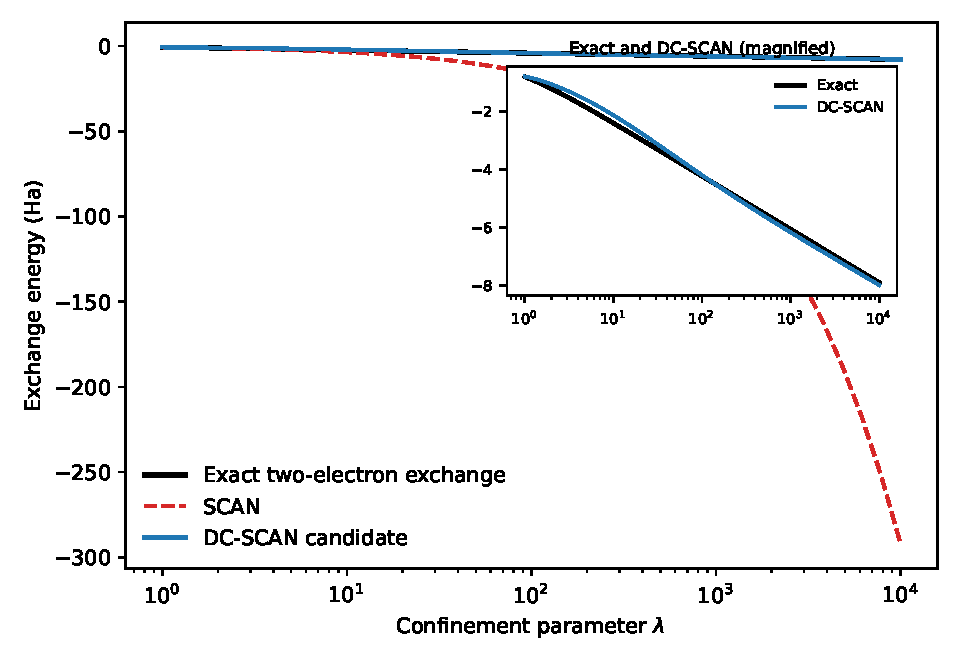
\includegraphics[width=0.8\linewidth]{scan1d2d_dcscan_wire_benchmark.pdf}
\caption{Exchange energy of the two-electron Gaussian wire against the
  confinement parameter $\lambda$: exact (eq~\href{main.pdf\#equation.11}{A11}), SCAN and
  DC-SCAN (eq~\href{main.pdf\#equation.20}{A20}).  SCAN diverges as a power of $\lambda$; the
  inset magnifies the exact and DC-SCAN curves and shows the residual offset
  of DC-SCAN.}
\label{fig:dcscan-wire}
\end{figure}

\section{Evaluation inside aniGTO}
\label{sec:dcscan-anigto}
The wire orbital $\phi=\sqrt{n_\lambda/2}$ is exactly the $s$ function of the
aniGTO harmonic-trap basis with $\boldsymbol\omega=(\lambda^2,\lambda^2,1)$,
whose exponents are $(\lambda^2/2,\lambda^2/2,1/2)$.  The aniGTO columns of
Table~\href{main.pdf\#table.1}{1} are computed with aniGTO objects only:
\begin{itemize}
\item the exact exchange is the aniGTO repulsion integral
  $-(\phi\phi|\phi\phi)$ of the trap molecule;
\item $n$, $\nabla n$, the Hessian $\nabla\nabla n$, $\nabla^2n$ and
  $\tau=\tfrac12\sum_if_i|\nabla\phi_i|^2$ are evaluated from analytic first and
  second derivatives of the aniGTO Cartesian Gaussians;
\item LDA, PBE, SCAN and r$^2$SCAN exchange are taken from libxc through PySCF,
  $F_x=e_x/e_x^{\mathrm{LDA}}$ pointwise, and $D$, $Z$, $s$ and $\alpha$
  (eqs~\href{main.pdf\#equation.4}{A4}, \href{main.pdf\#equation.5}{A5} and \href{main.pdf\#equation.18}{A18}) are formed on
  the grid from the aniGTO Hessian rather than from the closed form $C=A$.
\end{itemize}
On these one-orbital densities $|\alpha|\le10^{-8}$, and libxc SCAN and
r$^2$SCAN agree with the closed-form $\alpha=0$ branch (eq~\href{main.pdf\#equation.6}{A6})
to the printed digits.  As a second exact route, the quasi-1D Kantorovich
reduction gives $E_x=-\tfrac14\iint n(z)n(z')\,w_b(z-z')\,dz\,dz'$ with
$w_b(z)=\sqrt\pi/(2b)\,\mathrm{erfcx}(|z|/2b)$ and $b=1/(\sqrt2\lambda)$.  It is
exact here because both electrons share the transverse Gaussian, and it
reproduces eq~\href{main.pdf\#equation.11}{A11} to $10^{-15}$~Ha for all $\lambda$.

Table~\ref{tab:dcscan-anigto-grid} compares two grids.  The anisotropic
Gauss--Hermite product grid of the aniGTO DFT module, scaled per axis by the
smallest exponent, converges SCAN to $\le3\times10^{-3}$~Ha at every $\lambda$.
DC-SCAN, however, is switched on only in the region
$\lambda^{-2/3}\ll\lambda^2\rho^2\ll1$ that carries the wire logarithm, and that
region spans many decades in $\rho$.  A product grid uniform in $\rho$ cannot
resolve it, so for $\lambda\ge10^3$ DC-SCAN on that grid is not converged.  A
cylindrical grid, logarithmic in $u=\lambda^2\rho^2$ and $t=z$ (the coordinates of
eq~\href{main.pdf\#equation.33}{A33}) and evaluated at points of the aniGTO basis functions,
converges every entry to $10^{-7}$~Ha.  A Hessian-dependent functional thus
needs a logarithmic radial grid around the confinement axis before it can be
used self-consistently in aniGTO.

\begin{table}[H]
\centering
\caption{aniGTO evaluation of the wire exchange (hartree) on the Gauss--Hermite
  grid of the aniGTO DFT module (nodes per axis) and on the cylindrical
  logarithmic grid (Gauss--Legendre nodes per variable).  Computed values first:
  $N$ is the integrated electron number and the next seven columns are the
  exchange energies; then the differences: LDA, SCAN and DC-SCAN minus the
  reference quadrature of Table~\href{main.pdf\#table.1}{1}, and the closed-form
  SCAN ($\alpha=0$ branch) evaluated on the same grid minus libxc SCAN.}
\label{tab:dcscan-anigto-grid}
\scriptsize
\resizebox{\textwidth}{!}{%
\begin{tabular}{@{}rlrr|rrrrrrr|rrrr@{}}
\toprule
 & & & & \multicolumn{7}{c|}{computed values: aniGTO fields (eq~\ref{eq:ani-fields}), grid (eq~\ref{eq:ani-cyl}), libxc} & \multicolumn{4}{c}{differences} \\
$\lambda$ & grid & nodes & $N$ & LDA & PBE & SCAN & r$^2$SCAN & DC-SCAN & DC-PBE & DC-r$^2$SCAN &
  LDA$-$ref & SCAN$-$ref & DC-SCAN$-$ref & SCAN$^{\rm cf}-$SCAN \\
\midrule
10 & Gauss--Hermite & 80 & 2.00000000 & -3.165498 & -3.865468 & -3.649731 & -3.649731 & -2.126716 & -1.976367 & -2.126716 & +5.1e-14 & +3.3e-07 & +1.5e-04 & -4.4e-16 \\
10 & Gauss--Hermite & 160 & 2.00000000 & -3.165498 & -3.865468 & -3.649731 & -3.649731 & -2.126888 & -1.976753 & -2.126888 & +5.1e-14 & +4.4e-08 & -2.5e-05 & +0.0e+00 \\
10 & Gauss--Hermite & 240 & 2.00000000 & -3.165498 & -3.865468 & -3.649731 & -3.649731 & -2.126817 & -1.976674 & -2.126817 & +5.2e-14 & +6.5e-09 & +4.6e-05 & +0.0e+00 \\
10 & cylindrical log & 300 & 2.00000000 & -3.165498 & -3.865468 & -3.649731 & -3.649731 & -2.126863 & -1.976721 & -2.126863 & +9.4e-14 & +1.1e-13 & +7.6e-08 & +4.4e-16 \\
10 & cylindrical log & 400 & 2.00000000 & -3.165498 & -3.865468 & -3.649731 & -3.649731 & -2.126863 & -1.976722 & -2.126863 & +4.4e-16 & +1.8e-15 & +1.3e-15 & +0.0e+00 \\
10 & cylindrical log & 560 & 2.00000000 & -3.165498 & -3.865468 & -3.649731 & -3.649731 & -2.126863 & -1.976722 & -2.126863 & +8.1e-14 & +9.4e-14 & -3.2e-08 & +0.0e+00 \\
100 & Gauss--Hermite & 80 & 2.00000000 & -14.692939 & -20.817613 & -16.362346 & -16.362346 & -4.209902 & -4.014640 & -4.209902 & +2.3e-13 & -4.7e-05 & -1.6e-02 & +0.0e+00 \\
100 & Gauss--Hermite & 160 & 2.00000000 & -14.692939 & -20.817581 & -16.362302 & -16.362302 & -4.186642 & -3.984922 & -4.186642 & +2.3e-13 & -3.6e-06 & +7.2e-03 & -3.6e-15 \\
100 & Gauss--Hermite & 240 & 2.00000000 & -14.692939 & -20.817578 & -16.362299 & -16.362299 & -4.195736 & -3.994080 & -4.195736 & +2.3e-13 & -1.5e-07 & -1.9e-03 & +0.0e+00 \\
100 & cylindrical log & 300 & 2.00000000 & -14.692939 & -20.817577 & -16.362299 & -16.362299 & -4.193878 & -3.992240 & -4.193878 & +4.3e-13 & +4.8e-13 & -1.3e-10 & +0.0e+00 \\
100 & cylindrical log & 400 & 2.00000000 & -14.692939 & -20.817577 & -16.362299 & -16.362299 & -4.193878 & -3.992240 & -4.193878 & +0.0e+00 & -3.6e-15 & -1.8e-15 & +0.0e+00 \\
100 & cylindrical log & 560 & 2.00000000 & -14.692939 & -20.817577 & -16.362299 & -16.362299 & -4.193878 & -3.992240 & -4.193878 & +3.7e-13 & +4.1e-13 & -2.1e-11 & +0.0e+00 \\
1,000 & Gauss--Hermite & 80 & 2.00000000 & -68.198582 & -109.476193 & -70.764359 & -70.764359 & -7.158316 & -7.024959 & -7.158316 & +1.1e-12 & -1.4e-03 & -9.9e-01 & -2.8e-14 \\
1,000 & Gauss--Hermite & 160 & 2.00000000 & -68.198582 & -109.470731 & -70.763363 & -70.763363 & -6.161318 & -5.916625 & -6.161318 & +1.1e-12 & -4.0e-04 & +9.5e-03 & -1.4e-14 \\
1,000 & Gauss--Hermite & 240 & 2.00000000 & -68.198582 & -109.470303 & -70.763121 & -70.763121 & -6.022794 & -5.821126 & -6.022794 & +1.1e-12 & -1.6e-04 & +1.5e-01 & -2.8e-14 \\
1,000 & cylindrical log & 300 & 2.00000000 & -68.198582 & -109.470149 & -70.762964 & -70.762964 & -6.170789 & -5.965216 & -6.170789 & +2.0e-12 & +2.1e-12 & +9.9e-14 & -1.4e-14 \\
1,000 & cylindrical log & 400 & 2.00000000 & -68.198582 & -109.470149 & -70.762964 & -70.762964 & -6.170789 & -5.965216 & -6.170789 & -2.8e-14 & +1.4e-14 & -2.7e-15 & -2.8e-14 \\
1,000 & cylindrical log & 560 & 2.00000000 & -68.198582 & -109.470149 & -70.762964 & -70.762964 & -6.170789 & -5.965216 & -6.170789 & +1.7e-12 & +1.8e-12 & +1.0e-13 & -2.8e-14 \\
10,000 & Gauss--Hermite & 80 & 2.00000000 & -316.549776 & -546.118619 & -292.057294 & -292.057294 & -4.008572 & -4.061073 & -4.008572 & +5.0e-12 & +7.5e-03 & +4.0e+00 & -5.7e-13 \\
10,000 & Gauss--Hermite & 160 & 2.00000000 & -316.549776 & -545.687062 & -292.067275 & -292.067275 & -5.768257 & -5.915872 & -5.768257 & +4.9e-12 & -2.5e-03 & +2.2e+00 & -5.1e-13 \\
10,000 & Gauss--Hermite & 240 & 2.00000000 & -316.549776 & -545.622921 & -292.067066 & -292.067066 & -7.896087 & -7.982759 & -7.896087 & +5.1e-12 & -2.3e-03 & +9.4e-02 & -5.1e-13 \\
10,000 & cylindrical log & 300 & 2.00000000 & -316.549776 & -545.596537 & -292.064785 & -292.064785 & -7.990438 & -7.788276 & -7.990438 & +9.3e-12 & +9.2e-12 & +3.2e-13 & -4.5e-13 \\
10,000 & cylindrical log & 400 & 2.00000000 & -316.549776 & -545.596537 & -292.064785 & -292.064785 & -7.990438 & -7.788276 & -7.990438 & +5.7e-14 & +4.5e-13 & +8.9e-16 & -4.0e-13 \\
10,000 & cylindrical log & 560 & 2.00000000 & -316.549776 & -545.596537 & -292.064785 & -292.064785 & -7.990438 & -7.788276 & -7.990438 & +8.1e-12 & +7.7e-12 & +1.9e-13 & -4.0e-13 \\

\bottomrule
\end{tabular}}
\end{table}

\section{Gaussian sheet}
\label{sec:dcscan-sheet}
The sheet table of the main text (Table~\href{main.pdf\#table.2}{2}) uses
eq~\href{main.pdf\#equation.33}{A33} with $k=1$ and the same grid.  All eighteen exact, SCAN
and DC-SCAN entries agree with an independent evaluation to the six printed
decimals.  Raising the quadrature from 400 to 560 nodes changes DC-SCAN by at
most $7.6\times10^{-7}$~Ha (at $\lambda=2$) and SCAN by
$1.5\times10^{-13}$~Ha; widening the ranges to $u\le34$, $t\le10$, lower
limits $e^{-40}$, changes DC-SCAN by at most $2.7\times10^{-7}$~Ha.
Table~\ref{tab:dcscan-sheet-check} repeats the exact-exchange checks of
Table~\ref{tab:dcscan-check} for the sheet, with aniGTO exponents
$(1/2,1/2,\lambda^2/2)$.  Table~\ref{tab:dcscan-sheet-asym} follows the three
energies toward their $\lambda\to\infty$ limits.  The exact energy approaches
$-\sqrt{\pi/2}$ (eq~\href{main.pdf\#equation.12}{A12}) as $\sqrt{2/\pi}\,\lambda^{-1}$,
DC-SCAN$-$exact decays as $\lambda^{-1/3}$ (local exponent $-0.333$ over the
last decade), and SCAN approaches its own limit $-h_x^0a_1M_{2D}=-11.145141$~Ha
only as about $\lambda^{-0.23}$; that limit is reached only where
$s\gg a_1^2\approx24.5$ over most of the sheet.

\begin{table}[H]
\centering
\caption{Exact exchange of the Gaussian sheet and numerical checks (hartree),
  as in Table~\ref{tab:dcscan-check}; closed form eq~\href{main.pdf\#equation.10}{A10}.}
\label{tab:dcscan-sheet-check}
\scriptsize
\resizebox{\textwidth}{!}{%
\begin{tabular}{@{}r|rrrrrr|rrrr@{}}
\toprule
 & \multicolumn{6}{c|}{computed values} & \multicolumn{4}{c}{differences} \\
$\lambda$ & $E_x^{\mathrm{exact}}$, eq~\href{main.pdf\#equation.10}{A10} & eq~\href{main.pdf\#equation.44}{A44} & aniGTO, eq~\ref{eq:ani-eri-t} & aniGTO (fine), eq~\ref{eq:ani-eri-t} & $E_x^{\mathrm{DC}}$ (400) & $E_x^{\mathrm{DC}}$ (560) &
  eq~\href{main.pdf\#equation.44}{A44}$-$exact & aniGTO$-$exact & aniGTO (fine)$-$exact & $\Delta E^{\mathrm{DC}}_{400\to560}$ \\
\midrule
1 & -0.7978845608 & -0.7978845608 & -0.7978845608 & -0.7978845608 & -0.7950576394 & -0.7950576394 & $-6.1\times10^{-15}$ & $2.2\times10^{-16}$ & $0$ & $2.0\times10^{-14}$ \\
2 & -0.9648016727 & -0.9648016727 & -0.9648016727 & -0.9648016727 & -0.8693771541 & -0.8693763930 & $-2.2\times10^{-16}$ & $1.1\times10^{-16}$ & $1.1\times10^{-16}$ & $7.6\times10^{-7}$ \\
10 & -1.1793034311 & -1.1793034311 & -1.1793034311 & -1.1793034311 & -1.0829953753 & -1.0829953760 & $3.6\times10^{-14}$ & $4.4\times10^{-16}$ & $2.2\times10^{-16}$ & $-6.6\times10^{-10}$ \\
100 & -1.2453974301 & -1.2453974301 & -1.2453974301 & -1.2453974301 & -1.1847788041 & -1.1847788020 & $5.5\times10^{-14}$ & $0$ & $-1.1\times10^{-15}$ & $2.2\times10^{-9}$ \\
1,000 & -1.2525168789 & -1.2525168789 & -1.2525168789 & -1.2525168789 & -1.2214079455 & -1.2214079461 & $5.8\times10^{-14}$ & $-1.3\times10^{-15}$ & $-6.0\times10^{-15}$ & $-5.0\times10^{-10}$ \\
10,000 & -1.2532343551 & -1.2532343551 & -1.2533141435 & -1.2532343551 & -1.2385060219 & -1.2385060219 & $5.7\times10^{-14}$ & $-8.0\times10^{-5}$ & $-6.2\times10^{-14}$ & $6.9\times10^{-12}$ \\

\bottomrule
\end{tabular}}
\end{table}

\begin{table}[H]
\centering
\caption{Approach of the Gaussian sheet to the $\lambda\to\infty$ limits
  (hartree).  Computed values first ($E_x^{\mathrm{exact}}$, DC-SCAN, SCAN), then
  the differences: exact minus $-\sqrt{\pi/2}$, DC-SCAN minus exact, and SCAN
  minus its limit $-h_x^0a_1M_{2D}=-11.145141$.}
\label{tab:dcscan-sheet-asym}
\scriptsize
\begin{tabular}{@{}r|rrr|rrr@{}}
\toprule
 & \multicolumn{3}{c|}{computed values} & \multicolumn{3}{c}{differences} \\
$\lambda$ & $E_x^{\mathrm{exact}}$, eq~\href{main.pdf\#equation.10}{A10} & $E_x^{\mathrm{DC}}$, eq~\href{main.pdf\#equation.20}{A20} & $E_x^{\mathrm{SCAN}}$ & $E_x^{\mathrm{exact}}+\sqrt{\pi/2}$ & DC$-$exact & $E_x^{\mathrm{SCAN}}-E_\infty^{\mathrm{SCAN}}$ \\
\midrule
$10^{2}$ & -1.245397 & -1.184779 & -3.179886 & $7.9\times10^{-3}$ & +0.060619 & +7.9653 \\
$10^{2.5}$ & -1.250797 & -1.206554 & -4.128303 & $2.5\times10^{-3}$ & +0.044244 & +7.0168 \\
$10^{3}$ & -1.252517 & -1.221408 & -5.130958 & $8.0\times10^{-4}$ & +0.031109 & +6.0142 \\
$10^{3.5}$ & -1.253062 & -1.231573 & -6.121554 & $2.5\times10^{-4}$ & +0.021489 & +5.0236 \\
$10^{4}$ & -1.253234 & -1.238506 & -7.045312 & $8.0\times10^{-5}$ & +0.014728 & +4.0998 \\
$10^{4.5}$ & -1.253289 & -1.243228 & -7.866517 & $2.5\times10^{-5}$ & +0.010061 & +3.2786 \\
$10^{5}$ & -1.253306 & -1.246444 & -8.568654 & $8.0\times10^{-6}$ & +0.006862 & +2.5765 \\
$10^{5.5}$ & -1.253312 & -1.248634 & -9.150344 & $2.5\times10^{-6}$ & +0.004677 & +1.9948 \\
$10^{6}$ & -1.253313 & -1.250126 & -9.620105 & $8.0\times10^{-7}$ & +0.003187 & +1.5250 \\

\bottomrule
\end{tabular}
\end{table}

\subsection{Validation of the sheet construction against the literature}
\label{sec:lit-validation}
\novelty{In the $\lambda\to\infty$ (2D) limit of a one-orbital density, $s$ diverges, and any
enhancement factor with $F_x\to A\,s^{-1/2}$ gives the finite exchange energy
\begin{equation}
E_x\to-C_XA\,K\int n^2\,|\partial_zn|^{-1/2}\,d^3r,\qquad K=\bigl[2(3\pi^2)^{1/3}\bigr]^{1/2},
\label{eq:lit-limit}
\end{equation}
because $n^{4/3}s^{-1/2}=K\,n^2|\partial_zn|^{-1/2}$.  Fixing $A$ so that
eq~\ref{eq:lit-limit} equals the exact 2D limit gives the DC-SCAN sheet coefficient
$A_{2D}$ (eqs~\href{main.pdf\#equation.28}{A28}--\href{main.pdf\#equation.29}{A29}); setting $A=h_x^0a_1$ gives the
SCAN limit.  We applied the same formula, unchanged, to the infinite-barrier slab
\begin{equation}
n(z)=n_{2D}\,\frac{2}{L}\sin^2\frac{\pi z}{L},\quad n_{2D}=\frac{1}{\pi r_s^2},\qquad
\int n^2|n'|^{-1/2}dz=\frac{(2n_{2D})^{3/2}}{\sqrt2\,\pi^{3/2}}\,B\bigl(\tfrac94,\tfrac14\bigr),
\label{eq:lit-slab}
\end{equation}
with $B$ the Beta function.
It reproduces Constantin's coefficient $a_x$ for the exact 2D limit of the slab and
the SCAN 2D limit of Kaplan, Wagle and Perdew, both obtained independently
(Table~\ref{tab:lit-validation}); $a_x$ is independent of $r_s^{2D}$ to all printed
digits.  The remaining 0.9\% difference to the numerical SCAN value of
ref~\citenum{kaplan2018collapse} is that of their quadrature at
$L/r_s^{2D}=10^{-10}$ against our exact limit; their own analytic estimate agrees
to 0.02\%.}

\begin{table}[H]
\centering
\color{red}
\caption{\novelty{The sheet-limit construction of DC-SCAN (eq~\ref{eq:lit-limit}) applied to the
  infinite-barrier slab of refs~\citenum{constantin2008dimensional,kaplan2018collapse}
  and to the Gaussian sheet of this work.  aniGTO: the same quantity from the aniGTO exact
  exchange of the Gaussian sheet at $\lambda=10^8$ (eqs~\ref{eq:ani-Ik-s}--\ref{eq:ani-selfrep} in the
  logarithmic variable of eq~\href{main.pdf\#equation.1}{1}), $-1.253314129337$~Ha, equal to the closed form
  eq~\href{main.pdf\#equation.10}{A10} to 12 digits; ``--'': not applicable (the $\sin^2$ slab is not a
  Gaussian density).  Computed values first, then the literature or reference value, its
  source, and the relative differences at the end.}}
\label{tab:lit-validation}
\scriptsize
\resizebox{\textwidth}{!}{%
\begin{tabular}{@{}lrrrlrr@{}}
\toprule
 & \multicolumn{2}{c}{this work} & & & \multicolumn{2}{c}{difference to reference} \\
\cmidrule(lr){2-3}\cmidrule(l){6-7}
quantity & eq~\ref{eq:lit-limit} & aniGTO, eq~\ref{eq:ani-selfrep} & reference & source & eq~\ref{eq:lit-limit} & aniGTO \\
\midrule
slab: exact 2D $E_x/N$ (Ha), $r_s^{2D}=4$ & -0.150053 & -- & \href{https://doi.org/10.1103/PhysRevB.98.085147}{\textcolor{red}{-0.1501}} & ref~\citenum{kaplan2018collapse} & $+0.03$\% & -- \\
slab: $a_x$ giving the exact 2D limit & 0.521748 & -- & \href{https://doi.org/10.1103/PhysRevB.78.155106}{\textcolor{red}{0.5217}} & ref~\citenum{constantin2008dimensional}, eq~12 & $+0.01$\% & -- \\
slab: SCAN 2D limit $E_x/N$ (Ha), analytic & -1.670599 & -- & \href{https://doi.org/10.1103/PhysRevB.98.085147}{\textcolor{red}{-1.6710}} & ref~\citenum{kaplan2018collapse}, App.~A & $+0.02$\% & -- \\
slab: SCAN 2D limit $E_x/N$ (Ha), numerical & -1.670599 & -- & \href{https://doi.org/10.1103/PhysRevB.98.085147}{\textcolor{red}{-1.6550}} & ref~\citenum{kaplan2018collapse}, numerical & $-0.94$\% & -- \\
slab: SCAN/exact & 11.133411 & -- & \href{https://doi.org/10.1103/PhysRevB.98.085147}{\textcolor{red}{11.0260}} & ref~\citenum{kaplan2018collapse} & $+0.97$\% & -- \\
Gaussian sheet: exact 2D limit $E_x$ (Ha) & -1.253314 & -1.253314 & -1.2533 & eq~\href{main.pdf\#equation.12}{A12} & $+0.00$\% & $+0.00$\% \\
Gaussian sheet: $A_{2D}$ & 0.653226 & 0.653226 & 0.6532 & eq~\href{main.pdf\#equation.29}{A29} & $+0.00$\% & $-0.00$\% \\
Gaussian sheet: SCAN limit (Ha) & -11.145141 & -- & -11.1451 & eq~\href{main.pdf\#equation.28}{A28}, Table~\href{main.pdf\#table.2}{2} & $+0.00$\% & -- \\
Gaussian sheet: SCAN/exact & 8.892536 & 8.892536 & 8.8900 & main text & $+0.03$\% & $+0.03$\% \\

\bottomrule
\end{tabular}}
\end{table}


\begin{figure}[H]
\centering
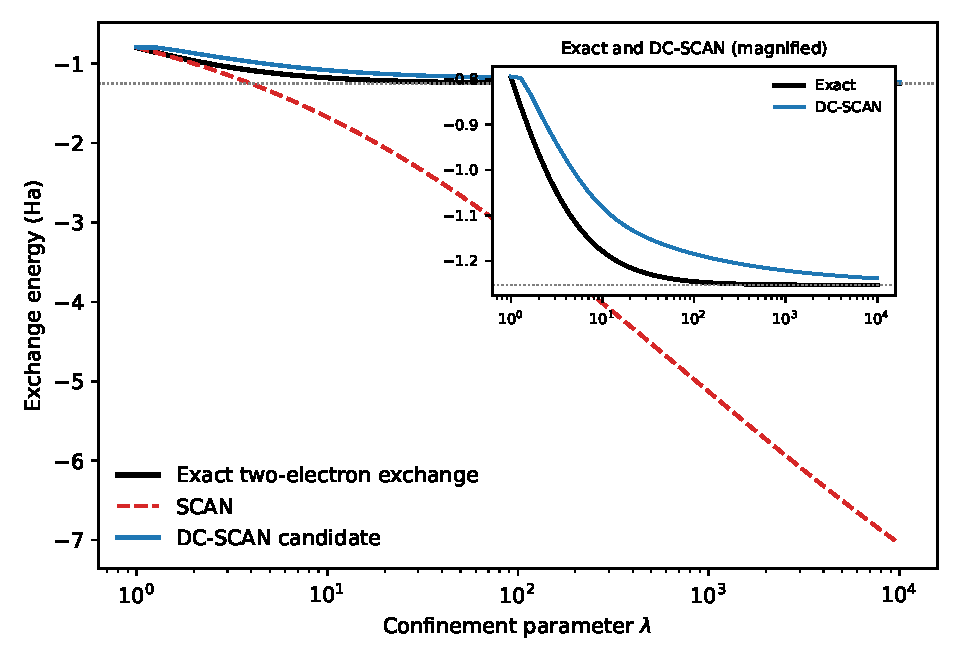
\includegraphics[width=0.8\linewidth]{scan1d2d_dcscan_sheet_benchmark.pdf}
\caption{Exchange energy of the two-electron Gaussian sheet against the
  confinement parameter $\lambda$: exact, SCAN and DC-SCAN
  (eq~\href{main.pdf\#equation.20}{A20}).  The dotted line is the exact limit $-\sqrt{\pi/2}$;
  the inset magnifies the exact and DC-SCAN curves.}
\label{fig:dcscan-sheet}
\end{figure}

\section{PBE base and refit of the activation scales}
\label{sec:dcscan-refit}
Replacing $F_x^{\mathrm{SCAN}}$ by the PBE enhancement factor in
eq~\href{main.pdf\#equation.20}{A20} (DC-PBE) keeps the sheet limit and the wire log
coefficient, since both are set by the dimensional branches.  PBE alone, whose
$F_x$ saturates at 1.804, grows like LDA.  The activation function
eq~\href{main.pdf\#equation.25}{A25} has two scales that the construction sets to one; it is
generalized here to
\begin{equation}
\Omega=\frac{(Z/Z_0)^3}{1+(Z/Z_0)^3}\,\frac{(s/s_0)^8}{1+(s/s_0)^8}.
\end{equation}
Any
$s_0,Z_0>0$ preserve the uniform-gas limit, the Gaussian sheet limit and the
wire log coefficient, because $A_{2D}$ and $A_{1D}$ are not changed.  Fitting
only $s_0$ and $Z_0$ to the wire errors at $\lambda=2$--$10^4$ and using the
sheet family as an independent test set gives Table~\ref{tab:dcscan-refit}.
The fit selects $s_0\approx1$ and $Z_0\approx2.3$ (SCAN) or 2.6 (PBE),
lowering the wire RMS error by a factor of 5--6.  The sheet errors, which
were not fitted, change by at most 0.08~Ha, and the sheet RMS improves.  This
is a two-parameter, one-family fixed-density fit, reported as a diagnostic of
where the remaining finite-width error comes from, not as a validated
parametrization.

\begin{table}[H]
\centering
\caption{Exchange energies $E_x$ and errors $E_x-E_x^{\mathrm{exact}}$ (hartree) of
  the base functionals, DC-SCAN/DC-PBE with unit activation scales, and the
  wire-fitted scales $(s_0,Z_0)$, on the wire (fit set) and the sheet (test set).
  The exact closed-form values come first, then for every variant the computed
  $E_x$, and the errors and their RMS at the end of the row.}
\label{tab:dcscan-refit}
\scriptsize
\resizebox{\linewidth}{!}{%
\begin{tabular}{@{}ll|rrrrr|rrrrrr@{}}
\toprule
 & & \multicolumn{5}{c|}{$E_x$ (Ha)} & \multicolumn{6}{c}{$E_x-E_x^{\mathrm{exact}}$ (Ha)} \\
variant & family & $\lambda=2$ & 10 & 100 & $10^3$ & $10^4$ & $\lambda=2$ & 10 & 100 & $10^3$ & $10^4$ & RMS \\
\midrule
exact, eq~\href{main.pdf\#equation.11}{A11} & wire & -1.213337 & -2.400278 & -4.227637 & -6.064646 & -7.901840 &  &  &  &  &  &  \\
exact, eq~\href{main.pdf\#equation.10}{A10} & sheet & -0.964802 & -1.179303 & -1.245397 & -1.252517 & -1.253234 &  &  &  &  &  &  \\
\midrule
SCAN alone & wire & -1.260632 & -3.649731 & -16.362299 & -70.762964 & -292.064785 & -0.0473 & -1.2495 & -12.1347 & -64.6983 & -284.1629 & 130.4479 \\
SCAN alone & sheet & -1.000228 & -1.672690 & -3.179886 & -5.130958 & -7.045312 & -0.0354 & -0.4934 & -1.9345 & -3.8784 & -5.7921 & 3.2428 \\
DC-SCAN ($s_0=Z_0=1$) & wire & -1.060136 & -2.126863 & -4.193878 & -6.170789 & -7.990438 & +0.1532 & +0.2734 & +0.0338 & -0.1061 & -0.0886 & 0.1539 \\
DC-SCAN ($s_0=Z_0=1$) & sheet & -0.869388 & -1.082998 & -1.184779 & -1.221408 & -1.238506 & +0.0954 & +0.0963 & +0.0606 & +0.0311 & +0.0147 & 0.0682 \\
DC-SCAN refit ($s_0=0.986$, $Z_0=2.291$) & wire & -1.159757 & -2.410988 & -4.224040 & -6.083858 & -7.885874 & +0.0536 & -0.0107 & +0.0036 & -0.0192 & +0.0160 & 0.0269 \\
DC-SCAN refit ($s_0=0.986$, $Z_0=2.291$) & sheet & -0.927575 & -1.087504 & -1.181895 & -1.220053 & -1.237878 & +0.0372 & +0.0918 & +0.0635 & +0.0325 & +0.0154 & 0.0550 \\
PBE alone & wire & -1.225359 & -3.865468 & -20.817577 & -109.470149 & -545.596537 & -0.0120 & -1.4652 & -16.5899 & -103.4055 & -537.6947 & 244.9839 \\
PBE alone & sheet & -0.974775 & -1.890956 & -5.067933 & -11.945449 & -26.332795 & -0.0100 & -0.7117 & -3.8225 & -10.6929 & -25.0796 & 12.3162 \\
DC-PBE ($s_0=Z_0=1$) & wire & -0.983007 & -1.976722 & -3.992240 & -5.965216 & -7.788276 & +0.2303 & +0.4236 & +0.2354 & +0.0994 & +0.1136 & 0.2493 \\
DC-PBE ($s_0=Z_0=1$) & sheet & -0.811207 & -1.021854 & -1.152074 & -1.205856 & -1.231250 & +0.1536 & +0.1574 & +0.0933 & +0.0467 & +0.0220 & 0.1093 \\
DC-PBE refit ($s_0=1.013$, $Z_0=2.622$) & wire & -1.113806 & -2.420413 & -4.219246 & -6.074800 & -7.896149 & +0.0995 & -0.0201 & +0.0084 & -0.0102 & +0.0057 & 0.0459 \\
DC-PBE refit ($s_0=1.013$, $Z_0=2.622$) & sheet & -0.890883 & -1.043359 & -1.155006 & -1.207227 & -1.231886 & +0.0739 & +0.1359 & +0.0904 & +0.0453 & +0.0213 & 0.0832 \\

\bottomrule
\end{tabular}}
\end{table}

\section{Beyond the semilocal form: range separation, a quasi-1D LDA and local hybrids}
\label{sec:dcscan-beyond}
All results below are fixed-density (fixed-orbital), exchange-only and
exploratory; errors are $E_x-E_x^{\mathrm{exact}}$ in mHa.

\emph{Range separation.}  With $\mathrm{erf}(\omega r)/r=(2/\sqrt\pi)
\int_0^\omega e^{-t^2r^2}dt$, the exact long-range part is
eq~\href{main.pdf\#equation.44}{A44} with upper limit $\omega$.  At the HSE06 value
$\omega=0.11$ the short-range part carries 90\% ($\lambda=2$) to 98\%
($\lambda=10^4$) of the wire exchange, so replacing 25\% of it by HF only
scales the error: HSE06-type DC-SCAN (short-range DFA through the ITYH
attenuation\cite{iikura2001long}) gives $+119$, $+220$, $+50$, $-50$ and
$-36$ for $\lambda=2$, 10, 100, $10^3$, $10^4$.  Long-range-corrected forms
cannot remove the SCAN divergence, which comes from the short-range region
near the axis, and the ITYH attenuation, calibrated on the 3D uniform gas,
spoils the DC branches (LC-DC-SCAN with $\omega=1$: $-990$ at $\lambda=10^4$).

\emph{Quasi-1D LDA.}  For a product density $n_1(z)g_b(\rho)$ with a
Gaussian transverse profile, the exchange of the 1D uniform gas with the
transverse-averaged interaction $w_b$ is
\begin{equation}
e_x^{1D}(n_1)=-2\int_0^\infty\Bigl[\frac{\sin(kr)}{\pi r}\Bigr]^2w_b(r)\,dr,\qquad
w_b(x)=\frac{\sqrt\pi}{2b}\,\mathrm{erfcx}\Bigl(\frac{|x|}{2b}\Bigr),\qquad k=\frac{\pi n_1}{2},
\end{equation}
and the local functional $E_x^{\mathrm{q1D}}=\int e_x^{1D}(n_1(z))\,dz$ uses
$b=(2C_\perp)^{-1/2}$ from the density curvature (eq~\href{main.pdf\#equation.16}{A16}).  On the
Gaussian wire its errors are $+90.3$, $+116.5$, $+120.2$, $+120.2$, $+120.2$:
the logarithm is exact and what remains is a $\lambda$-independent error of
the axial inhomogeneity.  Because the Kantorovich expression
$E_x=-\frac14\iint n_1(z)n_1(z')w_b(z-z')\,dz\,dz'$ is exact for every
two-electron product density, the transferability of a correction can be
tested on other axial profiles (Table~\ref{tab:dcscan-q1d}).  A 1D gradient
term $-c\int n_1^2h(s_1)\,dz$, $s_1=|n_1'|/n_1^2$, $h=s^2/(1+s^2)$,
$c=0.1959$ fitted on the Gaussian, reaches 0.03~mHa on the Gaussian and on a
three times wider Gaussian, but not on other shapes, and it cannot describe
one orbital spread over two lobes, whose inter-lobe exchange is nonlocal.

\begin{table}[H]
\centering
\caption{Quasi-1D LDA and the Gaussian-fitted 1D GGA on two-electron wires with
  different axial profiles $n_1(z)$ (normalized to 2), $\lambda=10^3$.  Computed
  exchange energies first (Ha; exact from the Kantorovich expression), then the
  errors of q1D-LDA and q1D-GGA (mHa).}
\label{tab:dcscan-q1d}
\scriptsize
\begin{tabular}{@{}l|rrr|rr@{}}
\toprule
 & \multicolumn{3}{c|}{$E_x$ (Ha)} & \multicolumn{2}{c}{error (mHa)} \\
$n_1(z)\propto$ & exact, eq~\ref{eq:ani-kantorovich} & q1D-LDA & q1D-GGA & q1D-LDA & q1D-GGA \\
\midrule
$e^{-z^2}$ (fit) & $-6.06465$ & $-5.94441$ & $-6.06462$ & $+120.2$ & $+0.03$ \\
$e^{-z^2/9}$ & $-2.31374$ & $-2.27366$ & $-2.31373$ & $+40.1$ & $+0.01$ \\
$\mathrm{sech}^2z$ & $-5.17175$ & $-5.06758$ & $-5.17851$ & $+104.2$ & $-6.75$ \\
$e^{-z^4}$ & $-6.91797$ & $-6.81670$ & $-6.90579$ & $+101.3$ & $+12.17$ \\
$(1+z^2)^{-2}$ & $-5.99886$ & $-5.87876$ & $-6.02237$ & $+120.1$ & $-23.51$ \\
$e^{-(z-1.5)^2}+e^{-(z+1.5)^2}$ & $-3.25469$ & $-3.28592$ & $-3.37617$ & $-31.2$ & $-121.48$ \\
$z^2e^{-z^2}$ & $-4.54849$ & $-4.63594$ & $-4.76564$ & $-87.5$ & $-217.16$ \\

\bottomrule
\end{tabular}
\end{table}

\emph{Local hybrids and $N>2$.}  The local hybrid
$E_x^{\mathrm{LH}}=\int[a\,e_x^{\mathrm{HF}}+(1-a)\,e_x^{\mathrm{DFA}}]\,d^3r$
with the iso-orbital weight $a=\tau_W/\tau$\cite{jaramillo2003local} is exact
for every one-orbital density ($a\equiv1$).  To test it beyond $N=2$, the
$N=4$ and $N=6$ wires occupy $\phi_k=g(\rho)h_k(z)$, $k<N/2$, with $g$ the
transverse Gaussian and $h_k$ the Hermite functions, i.e.\ the $s$, $p_z$ and
$d_{zz}$ functions of the aniGTO trap basis with
$\boldsymbol\omega=(\lambda^2,\lambda^2,1)$.  The conventional exchange-energy
density $e_x^{\mathrm{HF}}(\mathbf r)=-\sum_{ij}\phi_i\phi_j(\mathbf r)
\int\phi_i\phi_j(\mathbf r')|\mathbf r-\mathbf r'|^{-1}d^3r'$ is evaluated with
the Gaussian transform of $1/r$ (eq~\href{main.pdf\#equation.43}{A43}), which for these
anisotropic Gaussian products reduces to a one-dimensional $t$ integral with
closed-form Gaussian moments; it integrates to the Kantorovich exact exchange
to $3\times10^{-7}$~Ha.  The DFA energy densities come from libxc on a
cylindrical logarithmic grid; DC-SCAN uses the full
$F_x^{\mathrm{SCAN}}(s,\alpha)$ (eqs~\href{main.pdf\#equation.38}{A38}--\href{main.pdf\#equation.42}{A42})
and reproduces Table~\href{main.pdf\#table.1}{1} for $N=2$ to all printed digits.
Table~\ref{tab:dcscan-lh} shows that the local hybrids converge to the exact
exchange as $\lambda$ grows, because the transverse kinetic energy, identical
in $\tau$ and $\tau_W$, dominates and $\langle1-a\rangle_n$ falls roughly as
$\lambda^{-2}$.  At $\lambda\le100$ the errors are still 17--250~mHa.
DC-SCAN alone, whose 1D branch is fixed on $N=2$, misses by $-0.44$ ($N=4$)
and $-0.93$~Ha ($N=6$) at $\lambda=10^4$.

\begin{table}[H]
\centering
\caption{Exchange energies (Ha) and errors (mHa) of SCAN, DC-SCAN and of local
  hybrids ($a=\tau_W/\tau$) on $N$-electron Gaussian wires built from the aniGTO
  trap functions.  For each $N$ the computed values come first (exact, then every
  method), followed by the errors;
  $\langle1-a\rangle_n$ is the density-weighted mean of $1-a$.  For $N=2$
  every local hybrid is exact ($0.000$).}
\label{tab:dcscan-lh}
\scriptsize
\begin{tabular}{@{}llrrrrr@{}}
\toprule
$N$ & & $\lambda=2$ & 10 & 100 & $10^3$ & $10^4$ \\
\midrule
4 & $E_x^{\mathrm{exact}}$, eq~\ref{eq:ani-eed} (Ha) & $-2.714648$ & $-5.825266$ & $-10.828612$ & $-15.879898$ & $-20.932175$ \\
  & SCAN $E_x$ (Ha) & $-2.793642$ & $-8.222728$ & $-37.068321$ & $-161.286391$ & $-670.385083$ \\
  & DC-SCAN $E_x$ (Ha) & $-2.451291$ & $-5.238404$ & $-10.834946$ & $-16.348922$ & $-21.374615$ \\
  & LH-PBE $E_x$ (Ha) & $-2.697921$ & $-5.898669$ & $-10.848097$ & $-15.881711$ & $-20.932300$ \\
  & LH-SCAN $E_x$ (Ha) & $-2.761750$ & $-5.928513$ & $-10.850780$ & $-15.881846$ & $-20.932304$ \\
  & LH-DC-SCAN $E_x$ (Ha) & $-2.737362$ & $-5.911570$ & $-10.847641$ & $-15.881520$ & $-20.932279$ \\
  & $\langle1-a\rangle_n$ & $2.1\times10^{-1}$ & $2.6\times10^{-2}$ & $5.6\times10^{-4}$ & $8.6\times10^{-6}$ & $1.2\times10^{-7}$ \\
  & SCAN error (mHa) & $-79.0$ & $-2397.5$ & $-26239.7$ & $-145406.5$ & $-649452.9$ \\
  & DC-SCAN error (mHa) & $+263.4$ & $+586.9$ & $-6.3$ & $-469.0$ & $-442.4$ \\
  & LH-PBE error (mHa) & $+16.7$ & $-73.4$ & $-19.5$ & $-1.81$ & $-0.125$ \\
  & LH-SCAN error (mHa) & $-47.1$ & $-103.2$ & $-22.2$ & $-1.95$ & $-0.129$ \\
  & LH-DC-SCAN error (mHa) & $-22.7$ & $-86.3$ & $-19.0$ & $-1.62$ & $-0.104$ \\
\midrule
6 & $E_x^{\mathrm{exact}}$, eq~\ref{eq:ani-eed} (Ha) & $-4.348090$ & $-9.820593$ & $-18.912057$ & $-28.124097$ & $-37.338748$ \\
  & SCAN $E_x$ (Ha) & $-4.439738$ & $-13.222856$ & $-59.804103$ & $-261.133034$ & $-1089.992571$ \\
  & DC-SCAN $E_x$ (Ha) & $-3.982874$ & $-8.856365$ & $-18.916708$ & $-29.066547$ & $-38.266912$ \\
  & LH-PBE $E_x$ (Ha) & $-4.305669$ & $-9.991177$ & $-18.965500$ & $-28.129277$ & $-37.339110$ \\
  & LH-SCAN $E_x$ (Ha) & $-4.438678$ & $-10.070617$ & $-18.973239$ & $-28.129682$ & $-37.339123$ \\
  & LH-DC-SCAN $E_x$ (Ha) & $-4.384159$ & $-10.027305$ & $-18.964633$ & $-28.128757$ & $-37.339051$ \\
  & $\langle1-a\rangle_n$ & $3.1\times10^{-1}$ & $4.4\times10^{-2}$ & $9.9\times10^{-4}$ & $1.6\times10^{-5}$ & $2.1\times10^{-7}$ \\
  & SCAN error (mHa) & $-91.6$ & $-3402.3$ & $-40892.0$ & $-233008.9$ & $-1052653.8$ \\
  & DC-SCAN error (mHa) & $+365.2$ & $+964.2$ & $-4.7$ & $-942.5$ & $-928.2$ \\
  & LH-PBE error (mHa) & $+42.4$ & $-170.6$ & $-53.4$ & $-5.18$ & $-0.362$ \\
  & LH-SCAN error (mHa) & $-90.6$ & $-250.0$ & $-61.2$ & $-5.58$ & $-0.375$ \\
  & LH-DC-SCAN error (mHa) & $-36.1$ & $-206.7$ & $-52.6$ & $-4.66$ & $-0.303$ \\

\bottomrule
\end{tabular}
\end{table}

\section{Scope of the test}
\label{sec:dcscan-scope}
The coefficients follow from Gaussian reference profiles and are not exact
constants of the exchange functional for arbitrary sheet or wire densities.
The sheet and wire benchmarks use one Gaussian profile each;
three-dimensional norms (H, He, Ne, jellium), other confinement profiles and
self-consistent tests remain to be done, and the refit of
Table~\ref{tab:dcscan-refit} has to be tested on those before it can be
trusted; Hessian-level meta-GGAs have been implemented
self-consistently elsewhere\cite{dabbaghi2026hessian}.

\section{Standalone codes}
\label{sec:codes}
Every number and figure of the main text and this SI is produced by one of
eight standalone Python scripts in the folder \texttt{codes/}.  Each script is
a single file that defines every function it uses (the DC-SCAN functional of
Appendix~\href{main.pdf\#section*.6}{A}, the aniGTO integrals of
Section~\ref{sec:anigto-derivation} copied verbatim from aniGTO, the
Kantorovich kernel and the SCE solver) and imports only numpy, scipy,
pandas, matplotlib and, where libxc is needed, PySCF.  A single command such
as \texttt{python3 01\_wire\_benchmark.py} writes its results to
\texttt{codes/results/} and its figures to \texttt{codes/figures/}.
\begin{table}[H]
\centering
\caption{Standalone scripts, the manuscript items they produce, and typical
  laptop run times.}
\label{tab:codes}
\scriptsize
\begin{tabular}{@{}llr@{}}
\toprule
script & produces & time \\
\midrule
\texttt{01\_wire\_benchmark.py} & Tables~\ref{tab:dcscan-check}--\ref{tab:dcscan-offset}, Figure~\ref{fig:dcscan-wire} & 3~min \\
\texttt{02\_sheet\_benchmark.py} & Table~\href{main.pdf\#table.2}{2}, Tables~\ref{tab:dcscan-sheet-check}, \ref{tab:dcscan-sheet-asym}, Figure~\ref{fig:dcscan-sheet} & 2~min \\
\texttt{03\_anigto\_wire\_libxc.py} & Table~\href{main.pdf\#table.1}{1}, Table~\ref{tab:dcscan-anigto-grid} & 2~min \\
\texttt{04\_exact\_vs\_proposed.py} & Table~\href{main.pdf\#table.4}{4}, Figure~\href{main.pdf\#figure.caption.5}{1} & 5~min \\
\texttt{05\_refit\_switch\_scales.py} & Table~\ref{tab:dcscan-refit} & 1~min \\
\texttt{06\_range\_separation\_q1d\_lda.py} & range separation and quasi-1D LDA (Section~\ref{sec:dcscan-beyond}) & $<1$~min \\
\texttt{07\_q1d\_gga\_profiles.py} & Table~\ref{tab:dcscan-q1d} & 1~min \\
\texttt{08\_local\_hybrid\_wires.py} & Table~\ref{tab:dcscan-lh} & 2~min \\
\bottomrule
\end{tabular}
\end{table}

\FloatBarrier
% compiled bibliography inlined; no BibTeX run needed
\providecommand{\latin}[1]{#1}
\makeatletter
\providecommand{\doi}
  {\begingroup\let\do\@makeother\dospecials
  \catcode`\{=1 \catcode`\}=2 \doi@aux}
\providecommand{\doi@aux}[1]{\endgroup\texttt{#1}}
\makeatother
\providecommand*\mcitethebibliography{\thebibliography}
\csname @ifundefined\endcsname{endmcitethebibliography}
  {\let\endmcitethebibliography\endthebibliography}{}
\begin{mcitethebibliography}{7}
\providecommand*\natexlab[1]{#1}
\providecommand*\mciteSetBstSublistMode[1]{}
\providecommand*\mciteSetBstMaxWidthForm[2]{}
\providecommand*\mciteBstWouldAddEndPuncttrue
  {\def\EndOfBibitem{\unskip.}}
\providecommand*\mciteBstWouldAddEndPunctfalse
  {\let\EndOfBibitem\relax}
\providecommand*\mciteSetBstMidEndSepPunct[3]{}
\providecommand*\mciteSetBstSublistLabelBeginEnd[3]{}
\providecommand*\EndOfBibitem{}
\mciteSetBstSublistMode{f}
\mciteSetBstMaxWidthForm{subitem}{(\alph{mcitesubitemcount})}
\mciteSetBstSublistLabelBeginEnd
  {\mcitemaxwidthsubitemform\space}
  {\relax}
  {\relax}

\bibitem[Chirchir \latin{et~al.}(2026)Chirchir, Jana, and
  {'S}miga]{chirchir2026anigto}
Chirchir,~G.; Jana,~S.; {'S}miga,~S. An Anisotropic Gaussian Integral Package
  for Quasi-Dimensional Quantum-Chemical Simulations. 2026; Manuscript in
  preparation\relax
\mciteBstWouldAddEndPuncttrue
\mciteSetBstMidEndSepPunct{\mcitedefaultmidpunct}
{\mcitedefaultendpunct}{\mcitedefaultseppunct}\relax
\EndOfBibitem
\bibitem[Kaplan \latin{et~al.}(2018)Kaplan, Wagle, and
  Perdew]{kaplan2018collapse}
Kaplan,~A.~D.; Wagle,~K.; Perdew,~J.~P. Collapse of the electron gas from three
  to two dimensions in {Kohn-Sham} density functional theory. \emph{Phys. Rev.
  B} \textbf{2018}, \emph{98}, 085147, DOI:
  \doi{10.1103/PhysRevB.98.085147}\relax
\mciteBstWouldAddEndPuncttrue
\mciteSetBstMidEndSepPunct{\mcitedefaultmidpunct}
{\mcitedefaultendpunct}{\mcitedefaultseppunct}\relax
\EndOfBibitem
\bibitem[Constantin(2008)]{constantin2008dimensional}
Constantin,~L.~A. Dimensional crossover of the exchange-correlation energy at
  the semilocal level. \emph{Phys. Rev. B} \textbf{2008}, \emph{78}, 155106,
  DOI: \doi{10.1103/PhysRevB.78.155106}\relax
\mciteBstWouldAddEndPuncttrue
\mciteSetBstMidEndSepPunct{\mcitedefaultmidpunct}
{\mcitedefaultendpunct}{\mcitedefaultseppunct}\relax
\EndOfBibitem
\bibitem[Iikura \latin{et~al.}(2001)Iikura, Tsuneda, Yanai, and
  Hirao]{iikura2001long}
Iikura,~H.; Tsuneda,~T.; Yanai,~T.; Hirao,~K. A long-range correction scheme
  for generalized-gradient-approximation exchange functionals. \emph{J. Chem.
  Phys.} \textbf{2001}, \emph{115}, 3540--3544, DOI:
  \doi{10.1063/1.1383587}\relax
\mciteBstWouldAddEndPuncttrue
\mciteSetBstMidEndSepPunct{\mcitedefaultmidpunct}
{\mcitedefaultendpunct}{\mcitedefaultseppunct}\relax
\EndOfBibitem
\bibitem[Jaramillo \latin{et~al.}(2003)Jaramillo, Scuseria, and
  Ernzerhof]{jaramillo2003local}
Jaramillo,~J.; Scuseria,~G.~E.; Ernzerhof,~M. Local hybrid functionals.
  \emph{J. Chem. Phys.} \textbf{2003}, \emph{118}, 1068--1073, DOI:
  \doi{10.1063/1.1528936}\relax
\mciteBstWouldAddEndPuncttrue
\mciteSetBstMidEndSepPunct{\mcitedefaultmidpunct}
{\mcitedefaultendpunct}{\mcitedefaultseppunct}\relax
\EndOfBibitem
\bibitem[Dabbaghi \latin{et~al.}(2026)Dabbaghi, Garc{\'i}a~Lastra, and
  de~Silva]{dabbaghi2026hessian}
Dabbaghi,~P.; Garc{\'i}a~Lastra,~J.~M.; de~Silva,~P. Self-consistent
  Hessian-level meta-generalized gradient approximation. \emph{Phys. Rev. B}
  \textbf{2026}, DOI: \doi{10.1103/x4qn-mbr1}\relax
\mciteBstWouldAddEndPuncttrue
\mciteSetBstMidEndSepPunct{\mcitedefaultmidpunct}
{\mcitedefaultendpunct}{\mcitedefaultseppunct}\relax
\EndOfBibitem
\end{mcitethebibliography}

\end{document}
